\chapter{Perceptual regimes of repetitive sound (PRiORS)}\label{sec:priors}

One of the crucial components that this project suggests is a general framework for modeling the dynamic mode of auditory perception and cognition: \emph{Perceptual Regimes of Repetitive Sound}, abbreviated as PRiORS. This framework is used here to account for phonological phenomena, i.e.~it is used to account for some cognitive aspects of auditory perception that are manifested in linguistic systems.
PRiORS reduces the rich acoustic signal to a single primitive, based solely on the notion of repetition, 
%i.e.~the reoccurrence of acoustic events in time, 
to account for auditory perception in terms of \emph{temporal integration}. Crucially, a major role is played by the \emph{rate} of repetitions, and , as PRiORS makes clear, this single quantitative modulation in rate of repetition has two qualitatively distinct effects in perception and cognition.

\section{Time and frequency dualism}\label{sec:dualism}

\subsection{Time and frequency domains in mathematical representations}\label{sec:dualismDomains}

Very often we are interested in representing and analyzing the course of certain observed phenomena over time. This relates to physical signals, mathematical functions and any time series of data such as economic and environmental developments.
These \emph{time domain} representations are relatively straightforward as they follow the progression of a single variable. Typically, time is plotted on the x-axis, showing progression in time from left to right, while the y-axis is used to plot the magnitude of the observed variable.
Time domain representations are therefore very informative with regard to the change in magnitude (or power) over time of a single variable.



\begin{figure}
% % % {\centering \includegraphics[width=1\linewidth]{figures/graphics-sineTime-1}}
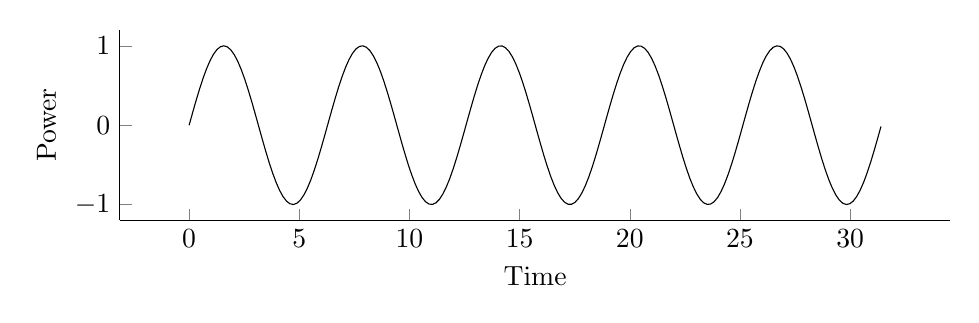
\begin{tikzpicture}
	\begin{axis}[
		axis lines*=left,
		width=\textwidth,
		height=4cm,
		ylabel=Power,
		xlabel=Time
		]
		\addplot [mark=none, black, domain=0:31.4, samples=200] {sin(deg(x))};
	\end{axis}
\end{tikzpicture}
\caption{An arbitrary sine wave in a time domain \emph{oscillogram} representation}\label{fig:sineTime}
\end{figure}

Time domain representations apply well to acoustic signals, where we can observe the progression of acoustic power over time to represent and analyze sounds.
In the simplest of cases, we can observe a single sine wave like the one in the oscillogram in \figref{fig:sineTime}. Here, a time domain representation is very informative with respect to the signal it depicts. The power, the (fundamental) frequency and the duration of the signal can all be readily deduced from this representation.
However, most natural sounds involve a much more complex distribution of acoustic power over different frequencies at different durations, many of them overlapping in time.
A time domain representation of complex natural sounds can effectively represent the overall impact of the many subcomponents on the amount of acoustic power at different points in time. It is, however, not very well suited to being informative with respect to any of the subcomponents of complex sound. Their individual frequencies, power and durations are all bundled together when we measure acoustic power over time.

We can decompose the complex signal into its subcomponents, provided that the subcomponents can be described as periodic signals, just like the simplest non-decomposable sine wave that characterizes acoustic signals. Doing that requires a switch from the time domain to the \emph{frequency domain}: rather than looking at the distribution of acoustic power over time, we can look at the distribution of acoustic power over different frequencies. A frequency domain representation allows us to observe the many subcomponents in terms of their frequency and power at given points in time.

Switching from time domain to frequency domain is possible with the \emph{Fourier transform}, a mathematical transform named after the French mathematician Jean-Baptiste-Joseph Fourier, who introduced it in \citet{fourier1822theoriesk}.
The Fourier transform decomposes a time series into a sum of finite series of sine or cosine functions.
Note that in many contexts of acoustic analysis, the procedure is referred to as \emph{fast Fourier transform} (FFT), which is the name given to a wide range of algorithms that perform quick calculations of the Fourier transform (see overview in \citealt{brigham1988fastsk}).

The time and frequency domains are two complementary, and, to some extent, redundant mathematical representations of the same physical reality.
By representing time as a scale of different potential rates, we can shift the representation of events in time into a representation of the co-activation of different rates in the frequency domain.
%It is perhaps useful to imagine the frequency domain as an interpretation of the time domain, whereby time is converted to one of its main effects -- the time-related impression of \emph{speed} (or \emph{rate}).
%Crucially, note that both domains are available for representation of physical events, regardless of timescales.

\subsection{Time and place theories in models of pitch perception}\label{sec:dualismPitch}

Models of pitch perception attempt to explain how the auditory system resolves the harmonic structure of complex signals into the sensation of pitch.
Two types of theories have traditionally dominated this field.
\emph{Place} theories of pitch are based on the idea that different frequencies in the signal can excite different places along the basilar membrane. \emph{Time} (or \emph{temporal}) theories of pitch are based on the idea that neural firing rates exhibit sensitivity in time to periodic events, allowing them to \emph{phase-lock} to the rate of periodicity in time.

Place theories of pitch often date back to \citet{ohm1843annalensk} and \citet{helmholtz1863lehresk}, and they are in line with the notion of the frequency domain (\citealt{ohm1843annalensk} in fact assumed that a Fourier analysis took place in the auditory system). Time theories of pitch often date back to \citet{seebeck1841annalensk, wever1930nature} and \citet{schouten1938perception}, and they are likewise in line with 
the notion of the time domain.
%time theories of pitch.
\citet{de2005pitch} traced back the early roots of these two pitch theories to ancient Greece, linking writings from Pythagoras (6th century BCE) and Aristoxenos (4th century BCE) with place theories of pitch, and linking the writings of Greek mathematician Nicomachus (2nd century CE) with time theories of pitch.

Place and time theories are sometimes presented as two dueling narratives, highlighting historical differences between \citet{seebeck1841annalensk} and \citet{ohm1843annalensk}, and later between \citet{helmholtz1863lehresk} and \citet{schouten1938perception} and many others. However, of consequence to this work is the more currently common appreciation that these two theories of pitch are, in fact, complementary and even desirably redundant to various extents (see \citealt{house1990tonal, de2005pitch, houtsma1995pitch, oxenham2013revisiting}).

\begin{sloppypar}
\citet{warren1981perception} mention the findings that frequency selectivity along the basilar membrane, which is essential for place-related pitch resolution, is roughly limited to 50--16k Hz \citep{bekesy1960experiments}, while phase-locking of the auditory nerve fibers' firing rate, which is essential for time-related pitch resolution, has a typical upper limit of about 5k Hz (\citealt{rose1967phase}; see a more recent review on this topic in \citealt{verschooten2019upper}).
\citet{warren1981perception} then make the point that the range in which both place and time models overlap, around 50--5k Hz is exactly the range for optimal perception of musical pitch.
\end{sloppypar}

\section{The spectral and temporal regimes of auditory perception}\label{sec:spectemp}

Auditory perception according to PRiORS is dramatically affected by two different responses to repetitions at two distinct timescales that constitute two perceptual regimes: the \emph{temporal regime} and the \emph{spectral regime}. The temporal regime designates the timescale at which humans can perceive successive acoustic events as isolated events in time, while exhibiting a relatively good ability to predict the upcoming event with a given steady rate, or perceive and estimate durations, in the related terminology of \citet{fraisse1984perception}. These upper and lower limits of perception were described in \citet[321]{macdougall1903structure} as conditions for \enquote{the impression of rhythm}, and, indeed, the timescale of the temporal regime defines the range at which musical rhythmic patterns tend to occur and auditory sensitivity to changes in rate allows us to reliably detect temporal patterns (e.g.~\citealt{fraisse1984perception, farbood2013temporal, repp2005sensorimotor}). In other words, the temporal regime covers our ability to perceive the difference between \emph{fast} and \emph{slow}.

The spectral regime, in contrast, operates at a faster timescale, where a sequence of acoustic events repeats too fast to be perceived as isolated events (see, e.g, \citealt{miller1948perception, broadbent1959auditory, efron1973conversation, hirsh1959auditory}). At these fast rates, rather than perceiving temporal intervals as occurring at non-overlapping moments in time, cognition switches to perceiving them as spectral intervals that occur at the same time, giving rise to the perception of a complex harmonic tone, whereby the harmonic partials reflect the rate of repetition in the spectral dimension (\citealt{flanagan1960pitch, stockhausen1959how, warren1982auditory}). Within the spectral regime, changes in rate of repetition of periodic signals are perceived as changes in pitch.
In other words, the spectral regime covers our ability to perceive the difference between \emph{high} and \emph{low} (pitch).\footnote{The notion of repetition is not limited to rate-based distinctions, but this work requires only this type of distinction to cover prosodic phenomena. To cover the acoustic qualities of segmental phenomena in speech we can analyze the lack of regular repetition at the spectral regime in at least two meaningful ways: (i) transient bursts are characteristic of speech sounds like \emph{stops} that exhibit a non-repeating signal (or more accurately, a critically damped signal); (ii) continuous yet irregular (asynchronous) repetitions within the timescale of the spectral regime are characteristic of \emph{aperiodic} noise that results from articulatory friction (e.g.~\emph{fricatives}).}

In principle, the temporal regime is congruent with the notion of \emph{time domain} and the spectral regime is congruent with the notion of \emph{frequency domain} (see \sectref{sec:dualismDomains}).
Likewise, the two regimes correspond to the two independent anatomical and neurological processes for pitch resolution that are also based on time and frequency representations (see \sectref{sec:dualismPitch}).
However, while the time and frequency domains can independently describe the same event in mathematical terms, and while place and time theories of pitch perception may be, to a large extent, complementary and redundant, the perceptual regimes in PRiORS operate at two slightly overlapping yet mostly distinct and mutually exclusive timescales.
Each perceptual regime responds to repetitions within its timescale such that a single quantitative modulation of the rate of repetition gives rise to qualitative differences in the sensation of rhythm (temporal regime), or, alternatively, the sensation of pitch (spectral regime).
In other words, the temporal and spectral regimes suggest a perceptual qualia perspective, whereby the two regimes are mutually exclusive.

This last point is reminiscent of Pattee's quote from \citet[21]{pattee2012lawssk}, which was given in \sectref{sec:compofmind}, and is partially repeated here:
\enquote{It appears that our artificial instruments have extended our senses beyond what our classical brains can model without cognitive dissonance.}
In that sense, the time and frequency domains in physics are revealed by our instruments as two overlapping representations, but in our mind, the temporal and spectral regimes are represented as two distinct and separate sensations.
To be clear, auditory perception can handle the two regimes at the same time, i.e.~process information with both rhythmic and periodic effects. The mutual exclusivity is in response to isolated events within their relevant timescale.

When evaluating PRiORS, it is useful to acknowledge how the auditory system is uniquely adapted to capturing reoccurrence in terms of repetition. \citet{chowning2001perceptual} suggests that the auditory system is far more sensitive than the visual system to differences in reoccurring structures. He reflects this ability in the visual system in terms of the capacity to detect minute differences in the spacing between otherwise identical objects (think of a typical \emph{spot the difference} puzzle as an example), essentially equating quasi-periodicity with quasi-symmetry.
\citet[267]{chowning2001perceptual} claims that the auditory system, unlike the visual system, \enquote{can readily detect a fraction of a percent of deviation from periodicity}.
This great sensitivity to repetition is linked in PRiORS to perceptual and cognitive aspects of an auditory system that is specialized in processing rhythm and pitch
as the two modes of auditory temporal integration.

\section{Visual FFT-based simulations}\label{sec:blitit}

It is useful to illustrate the distinction between perceptual regimes with a \emph{Band-Limited Impulse Train} (BLIT) synthesis that produces a train of transient acoustic bursts at adjustable rates.
Each burst is a single \emph{impulse}, which is the shortest electric burst a given system can produce, with equal power across the frequency scale (a perfect impulse has acoustic power over an infinite frequency range, but the impulses in a BLIT, as the name suggests, are band-limited to human hearing ranges, between approx. 20--20k Hz).\footnote{One major advantage of the BLIT synthesis concerns the minimal duration of impulses that allows the simulation to reduce confounding factors regarding burst duration. Longer bursts are expected to appear as more continuous at slower rates than comparable impulses because they fill a longer portion of the intervals between onsets of recurring events (i.e.~they have a longer \emph{tail}).}
The BLIT signal can be effectively visualized with standard FFT-based tools that convert signals between time domain and frequency domain representations (see \sectref{sec:dualism})

\tabref{tab:priorsTimeScales} presents a rough sketch of the relevant timescales of the two perceptual regimes. Within each regime the effects of repetition are named differently in order to maintain a distinction that attempts to be in-line with most common uses of these terms: it is \emph{Rhythm} when occurring within the timescale of the temporal regime vs.~\emph{Periodicity} when occurring within the timescale of the spectral regime. \tabref{tab:priorsTimeScales} also shows that these repetition-induced effects have boundaries. Repetitions within the temporal regime may be too slow to be perceived as rhythmic (\emph{infra-rhythmic} perception below 30 BPM; see \citealt{fraisse1984perception, farbood2013temporal}, and see overview of tapping literature in \citealt{repp2005sensorimotor}). Likewise, repetitions within the spectral regime may be too fast to be perceived as periodic (\emph{ultra-periodic} perception above 5k Hz, given that our auditory system can typically perceive frequencies up to 20k Hz, but our ability to sense discernible pitches does not typically exceed 5k Hz; see \citealt{ward1954subjective, attneave1971pitch}).%\footnote{To understand what it means that above 5k Hz we hear frequencies that do not support pitch perception it is useful to consider a comparison between a \emph{pure tone} (sine wave) at a given frequency and a \emph{white noise} signal that was band-pass filtered to very narrowly target the same frequency of the sine wave. The claim is that above 5k Hz the periodic sine wave and the aperiodic band-pass filtered noise will not sound very different from each other because our auditory system cannot detect the periodic structures at these fast rates .}


\begin{table}
\caption{\label{tab:priorsTimeScales}Perceptual regimes with corresponding effects and timescales (rough sketch). \textit{Note.} Hz = Hertz (repetitions per second); BPM = Beat Per Minute; ms = millisecond (duration of repeating intervals).}
\begin{tabular}{lcccc}
\lsptoprule
& & \multicolumn{3}{c}{{Timescales}}\\\cmidrule(lr){3-5}
Perceptual regimes & Effects & Hz & BPM & ms \\\midrule
Temporal & \multicolumn{1}{c}{\color{gray}Infra-rhythmic} & \multicolumn{1}{c}{\color{gray}0--0.5} & \multicolumn{1}{c}{\color{gray}0--30} & \multicolumn{1}{c}{\color{gray}∞--2k} \\
& \multicolumn{1}{c}{Rhythm} & \multicolumn{1}{c}{0.5--20} & \multicolumn{1}{c}{30--1200} & \multicolumn{1}{c}{2k--50} \\\midrule
Spectral & \multicolumn{1}{c}{Periodicity} & \multicolumn{1}{c}{20--5k} & \multicolumn{1}{c}{1200--300k} & \multicolumn{1}{c}{50--0.2} \\
& \multicolumn{1}{c}{\color{gray}Ultra-periodic} & \multicolumn{1}{c}{\color{gray}5k--20k} & \multicolumn{1}{c}{\color{gray}300k--1200k} & \multicolumn{1}{c}{\color{gray}0.2--0.05} \\
\lspbottomrule
\end{tabular}
\end{table}

Four examples are provided in \figref{fig:priors-blit}, each one with three corresponding visual panels. The bottom white panel presents a 1-second long waveform (\emph{oscillogram}) which shows the unipolar transient bursts produced by the BLIT synthesis in the time domain, going from left to right. The number of visible bursts within this 1-second interval corresponds to the rate of the BLIT in Hz. The two upper dark panels show FFT-based analyses exhibiting the dispersion of acoustic power across the audible frequency range in the frequency domain. The middle panel, often called a \emph{spectrograph}, exhibits a 2-dimensional representation of frequency (x-axis) and power (y-axis), while the top panel, which is typically called a \emph{spectrogram}, exhibits a 3-dimensional representation of frequency (x-axis), power (color) and time (y-axis). The frequency x-axes of the spectrograph and the spectrogram are perfectly aligned to facilitate the interpretation of the spectrograph in the middle as a \enquote{slice}, or a \enquote{still image} of the temporal representation in the spectrogram above it.



\begin{figure}
\includegraphics[width=1\linewidth]{extrenal_figures/blitCombScaled.png} 
\caption{Illustration of perceptual regimes with visual analyses of acoustic impulse trains (BLIT) at different rates and different domains (see text for details).}\label{fig:priors-blit}
\end{figure}

\figref{fig:priors-blit}(a) (top left) shows a clear rhythmic effect at 4\,Hz, indicated by four bursts in the bottom oscillogram panel. A single burst appears with equal power along the (band-limited) frequency range in the spectrograph, indicated by the fairly straight horizontal green line across the middle panel.
Note that the still image shown here captured a moment in time in which the power graph of the spectrograph was high. With rhythmic bursts, like the 4\,Hz BLIT in \figref{fig:priors-blit}(a), this graph goes visibly up and down over time. Above it, a succession of 10 impulses over a short period of time (about 2.5 seconds) is visible as isolated bursts, indicated by the horizontal lines going from bottom to top in the corresponding upper spectrogram panel.

In sharp contrast, \figref{fig:priors-blit}(d) (bottom right) clearly shows tonal behavior at 120\,Hz. There are, indeed, 120 bursts in the time-domain display of the bottom oscillogram panel, but the isolated bursts are no longer visible in the top spectrogram panel, i.e. there are no horizontal lines going from bottom to top across the upper panel (note that with the 2.5 second-long window of the spectrogram, 120 bursts per second should have resulted in 300 horizontal lines by comparison to \figref{fig:priors-blit}(a)).
The sensation of isolated discrete bursts transitions into a sensation of continuous sound in perception at these higher rates of repetition. This can be thought of as a smearing effect that occurs above a certain threshold. This perceptual effect is neatly reflected by the two FFT-based representations in \figref{fig:priors-blit}(d), which display a signal with the properties of a continuous sound that has a complex harmonic structure. The middle spectrograph panel shows a series of \enquote{bumps} along the green curve, from left to right, corresponding to a series of continuous energy \enquote{poles} in the vertical representations of the upper spectrogram panel. This is a harmonic series in which the rate of repetition of the BLIT synthesis is mapped onto the fundamental frequency (F0) of the continuous sound, which is also manifested in the distance between partials in the harmonic series.\footnote{The polarity of the impulses can also play a role with pitch perception at higher rates within the spectral regime, as demonstrated in \citet{flanagan1960pitch}. For this reason, I used only unipolar impulses for which the relationship between impulse rate and frequency rate is kept stable.} Specifically, the two FFT-based representations in \figref{fig:priors-blit}(d) show the harmonic partials in terms of continuous acoustic power at the frequencies 120\,Hz, 240\,Hz, 360\,Hz, 480\,Hz, etc.
This demonstrates that at this faster timescale of the spectral regime, the sensation of repetition feeds perceptual effects of continuity and pitch, rather than of discreteness and rhythm.

The switch between regimes does not occur at once. Between the temporal and the spectral regime, we can spot a transitional range in which effects of both rhythm and periodicity are present, but neither is strong enough to completely take over. This results in a less definitive effective sensation.
Figures~\ref{fig:priors-blit}(b--c) demonstrate this transitional range between the two distinct regimes that are illustrated by \figref{fig:priors-blit}(a) (for the temporal regime) and \figref{fig:priors-blit}(d) (for the spectral regime), as detailed above.

\figref{fig:priors-blit}(b) (top right) is especially well-suited for illustrating the indeterminacy of the transitional range. At a BLIT rate of 24\,Hz, the impulses seem to be too fast to support a rhythmic perception of discrete bursts, and, at the same time, too slow to support the perception of a continuous harmonic (pitch-bearing) sound. The upper spectrogram panel of \figref{fig:priors-blit}(b) shows a combination of both horizontal lines that reflect isolated events in time, going from bottom to top, as well as vertical lines that reflect the emerging harmonic structure of a continuous complex tone (visible also as corresponding energy fluctuations in the middle spectrograph panel).

\begin{table}
\caption{\label{tab:transitionalTimeScales}Rough sketch of perceptual regimes with corresponding effects and timescales (transitions included). \textit{Note.} Hz = Hertz (repetitions per second); BPM = Beat Per Minute; ms = millisecond (duration of repeating intervals).}
\begin{tabular}{lcccc}
\lsptoprule
& & \multicolumn{3}{c}{Timescales}\\\cmidrule(lr){3-5}
Perceptual regimes & Effects &  Hz & BPM & ms \\\midrule

Temporal & \multicolumn{1}{c}{\color{gray}Infra-rhythmic} & \multicolumn{1}{c}{\color{gray}0--0.5} & \multicolumn{1}{c}{\color{gray}0--30} & \multicolumn{1}{c}{\color{gray}∞--2k} \\
   & \multicolumn{1}{c}{Rhythm} & \multicolumn{1}{c}{0.5--12} & \multicolumn{1}{c}{30--720} & \multicolumn{1}{c}{2k--83.3} \\
   & \multicolumn{1}{c}{\color{gray}Ultra-rhythmic} & \multicolumn{1}{c}{\color{gray}12--20} & \multicolumn{1}{c}{\color{gray}720--1200} & \multicolumn{1}{c}{\color{gray}83.3--50} \\\midrule
Spectral & \multicolumn{1}{c}{\color{gray}Infra-periodic} & \multicolumn{1}{c}{\color{gray}20--50} & \multicolumn{1}{c}{\color{gray}1200--3k} & \multicolumn{1}{c}{\color{gray}50--20} \\
   & \multicolumn{1}{c}{Periodicity} & \multicolumn{1}{c}{50--5k} & \multicolumn{1}{c}{3k--300k} & \multicolumn{1}{c}{20--0.2} \\
   & \multicolumn{1}{c}{\color{gray}Ultra-periodic} & \multicolumn{1}{c}{\color{gray}5k--20k} & \multicolumn{1}{c}{\color{gray}300k--1200k} & \multicolumn{1}{c}{\color{gray}0.2--0.05} \\
\lspbottomrule
\end{tabular}
\end{table}

To consider the transitional phases between the two regimes, \tabref{tab:transitionalTimeScales} pres\-ents a slightly more elaborate sketch than \tabref{tab:priorsTimeScales}, with transitional phases at 12--50\,Hz. Essentially, this emphasizes the fact that the main effects -- rhythm sensation in the temporal regime and periodic sensation in the spectral regime -- are optimally achieved closer to the center of each perceptual regime.

Note that the visual effects of the FFT-based representations in \figref{fig:priors-blit} are calibrated to reflect human perception.\footnote{Here I use a commercial metering application, SpectraFoo by Metric Halo (version 4.2.3), with the default Analyzer depth setting of 4,096 points (10\,Hz). The BLIT synthesis and the oscillogram were produced with the sound design software Plogue Bidule (version 0.9766).} The shift from temporal to spectral regimes does not represent a change in any physical quality. Rather, it represents a perceptual threshold of a given system.
A different system that responds to higher rates of periodicities, such as, for example, models simulating the auditory system of barn owls (see \citealt{koppl1997phasesk}), will most probably require higher frequencies to adequately represent the shift from the temporal to the spectral regime. Importantly, higher frequencies will require higher resolutions before the temporal representation becomes too fast and eventually \enquote{smears} into the spectral one.

\section{A note about previous works}\label{a-note-about-previous-works-warren-and-rosen}

The ideas in PRiORS are not entirely new. For one, they are not based on any new data, but on established findings in the literature from the fields of acoustics, auditory perception, neuroscience and linguistics. More specifically, previous proposals were presented in the past for frameworks of perception that are, much like PRiORS, based on delineating the unique contribution of different timescales to auditory perception.
I will summarize two of these in the following.

\begin{sloppypar}
Richard Warren, who studied temporal integration in auditory perception quite extensively, sketched a model with different perceptual effects at different timescales in \citet{warren1981perception} and \citet[80--85]{warren1982auditory}. \citet{warren1981perception} determined that 50--5k Hz is the optimal timescale for pitch perception (\enquote{melodic pure pitch}), given that in this range, both place-based and time-based resolutions of pitch are available.
At faster rates of 5k--16k Hz, where only place-based pitch resolution may be available, an \enquote{amelodic pure pitch} perception takes over.
At slower rates, between 20--50\,Hz, with only time-based pitch resolution available, the \enquote{pure pitch} sensation changes to \enquote{noisy pitch}. Further down, below 20\,Hz, repetitions are considered by \citet{warren1981perception} as \emph{infrapitch}, as they are too slow to induce a sensation of pitch.
\citet{warren1981perception} follow \citet{guttman1963lower} in determining 0.5\,Hz as a rough lower floor for perceptual integration of acoustic events. This 0.5\,Hz floor of about 2 second-long intervals is commonly mentioned as the lower threshold of the human ability to keep isochronous rhythm or temporally integrate events (see \citealt{fraisse1984perception, farbood2013temporal, repp2005sensorimotor}).
\end{sloppypar}

Approaching auditory perception of speech from a more linguistic point of view, \citet{rosen1992temporal} presented a framework for describing temporal information in speech, which can also be considered as a precursor of the PRiORS framework.
In his framework, \citet{rosen1992temporal} divides perception into three \enquote{temporal features} at distinct timescales: \emph{envelope} (2--50\,Hz), \emph{periodicity} (50--500\,Hz) and \emph{fine-structure} (600--1k Hz). \emph{Envelope} covers mainly \enquote{tempo, rhythm} and \enquote{syllabicity}, while \emph{periodicity} covers mainly \enquote{stress}, \enquote{intonation} and \enquote{voicing} (see \cite[76]{rosen1992temporal}, in which other segmental qualities are also covered).

\section{Advantages of PRiORS}\label{advantages-of-priors}

The PRiORS framework is useful for understanding various phenomena in auditory cognition and in phonological systems. It can be useful for models of speech perception that consider the contribution of auditory perception and cognition to language systems, as was detailed in \chapref{sec:lingMod}, and especially \sectref{sec:missinglinks}.
The following subsections address two major points that PRiORS can greatly help to elucidate. In Section~\ref{sec:universal} I discuss how PRiORS can dispel a lot of the mystery surrounding the phonological notion of the \emph{syllable}, and in Section~\ref{sec:quasi} I discuss PRiORS' potential for uncovering the different functions that music and speech utilize when they wield the effect of \emph{rhythm} from the timescale of the temporal regime.

\subsection{Universal aspects of syllabic structure}\label{sec:universal}

\begin{figure}
\includegraphics[width=1\linewidth]{extrenal_figures/SyllableSinesExtended} 
\caption{Schematic illustration of the relationship between perceptual regimes and syllabic units, using the three canonical syllables of the English word \emph{syllable} (demonstrated with one possible underlying annotation). Segmental makeup, i.e.~\emph{sonority}, is related to the spectral regime with high-frequency (\emph{periodic}) oscillations within syllables, while syllabic speech rate is related to the temporal regime with low-frequency (\emph{rhythmic}) oscillations between syllables. The ratio between the low-frequency and high-frequency oscillations in this illustration is arbitrarily set to be 1:20. This is a realistic ratio for syllables such that if syllables are taken to have a typical duration of 200\,ms (5\,Hz), the high-frequency oscillation within it would reflect a typical F0 for adult males at 100\,Hz. For simplicity, this generalized illustration shows a single rate at each timescale with isochronous repetitions (see Section~\ref{sec:quasi} on the more complex picture regarding isochrony in speech).%rather than quasi-repetitive ones (see Section~\ref{sec:quasi}).
}\label{fig:syll-sines}
\end{figure}

Syllables are, first and foremost, abstract units of phonological systems and they do not easily lend themselves to consistent and straightforward phonetic explanations in terms of perception and/or articulation.
The PRiORS framework can do a lot of heavy lifting in this regard, by providing the baseline conditions that can explain the evolutionary trajectory of syllables. According to this analysis, syllables were shaped by selection to optimally take advantage of the two perceptual regimes:
carrying pitch in the spectral regime and giving rise to speech rate relations in the temporal regime
(see \citealt{rasanen2018pre} for a similar type of analysis).
In other words, syllables have an internal segmental makeup that is optimized to carry pitch in order to exploit the distinction between low vs.~high periodicity in the spectral regime, and, at the same time, they appear in sizes that allow the distance between them to give rise to speech rate effects in order to exploit the distinction between slow vs.~fast rates in the temporal regime.
\figref{fig:syll-sines} illustrates this state of affairs with a highly generalized schematic sketch of the slower rhythmic cycle between syllables and faster periodic cycles within syllables.

PRiORS can therefore explain the universality of the typical syllable size and the universality of the preferred segmental makeup in the syllabic nucleus, which is commonly measured in linguistic terms of \emph{sonority}.
In line with PRiORS, this work claims that sonority should be understood as a measure of pitch intelligibility, acting as a defining feature of syllabic nuclei.
Syllables therefore need to be long enough to allow a minimum amount of periods to be effectively perceived.
For example, a very low F0 of 50\,Hz, which repeats every 20\,ms, requires a minimum of 3 periods (60\,ms) to be perceived, while higher F0 values (which characterize most speech) repeat faster and require even shorter minimum intervals (\citealt{fyk1987duration, josephs1967thephysics}). It is of interest to note that the average duration of syllables is about 200\,ms (5\,Hz, 300\,BPM), which is enough for adequate perception of pitch, as well as being at the center of the temporal regime, where it is optimally situated to achieve speech rate effects from the distance between syllables.

\subsection{Speech is quasi-repetitive}\label{sec:quasi}

The notion of repetition implies identical intervals between occurrences over time, i.e.~repetition is taken to be \emph{isochronous} unless otherwise stated. It has long been noted that pitch-inducing speech sounds are in fact not fully-isochronous, but, rather, \emph{quasi-periodic}, as the pitch and its underlying periods are often unstable at some level.
The notion of quasi-repetitiveness is mostly used to refer to an inherent \emph{jitter} in the regularity of repeating patterns that prevent perfect isochrony. This level of jitter (or noise) in the voice is assumed to be perceptually negligible.
However, on top of that there is another -- much larger -- source of apparent instability in repetitive structures in speech.
Speech is dynamically changing all the time, in magnitudes that far exceed the levels of inherent jitter, in order to achieve perceptible goals and to effectively exploit the sensations of rhythm and pitch.

Consider for example the periods during a rising pitch contour, in which every period is shorter than the previous one.
These degrees of change do not hinder the perception of coherent pitch contours, demonstrating our specialized ability to perceive dynamically-changing pitch.
As long as these communicatively relevant pitch differences occur within the timescale of the spectral regime
(and follow basic Gestalt principles)
they invoke a reliable effect in perception.
It is exactly these dynamic changes in the rate of repetition that prosody seems to exploit in speech.

A similar behavior can be observed for rhythm in speech. Speech rates do not typically appear as isochronous within the rhythm-inducing timescale of the temporal regime (see  \citealt{turk2013speechsk} and \citealt{nolan2014speechsk}). This is the temporal range which is exploited in speech for its perceptible effect on speech rate in terms of slow vs.~fast.
Crucially, there are no strong reasons to assume that the effect of rhythm in speech is exploited for isochrony, as it is not clear what purpose this would serve in speech.
However, in order to achieve various prosodic goals such as phrasal demarcation, turn-taking management and prominence marking (among many others), asynchronous temporal relations are exploited within the scope of speech rate sensations. In other words, speech is also \emph{quasi-rhythmic} and dynamically changing at the timescale of the rhythm-inducing effects of the temporal regime in order to be effective for prosody.

Confusingly, speech makes a very different usage of the temporal regime when compared to music, which, more often than not seems to favor isochronous rhythmic patterns over meandering ones within the rhythm-inducing timescale.
Musical experiences tend towards isochronous rhythms, perhaps because of the powerful ability of the perception of isochrony to create a shared clock that can be synced across separate systems and human agents, whereby different people can couple sensorimotor oscillations between one another and experience \emph{entrainment} (see, e.g., \citealt{cummins2009rhythm, cummins2015rhythm, benichov2016finding, haegens2018rhythmic, kotz2018evolution, rouse2016beat, tal2017neural}).

In contrast to a classic case of entrainment to external clocks, languages seem to use the effects of rhythm in the temporal regime for a different set of goals that do not seem to require isochrony and should not be considered to reflect classic entrainment (see, e.g., \citealt{cummins2012oscillators} and \citealt{meyer2019synchronous}).
%(see also \cite[1]{cummins2012oscillators}, on speech being insufficiently isochronous to support entrainment). 
The rhythm-inducing timescale is mostly used in speech to effectively exploit the distinction between slow and fast speech rates as useful cues in a system of speech prosody.
To that end, 
(quasi-)isochrony
%the most (quasi-)isochronus element 
in speech perception should be considered as internal (\textit{endogenous} neural activity) rather than external (\textit{exogenous} neural activity), to allow the hearer to infer the dynamic (and largely unpredictable) changes in the speech rate of their interlocutors.

%In other words, isochrony is not to be found 
%%(i.e. not 
%in the speech signal itself but in the mind of the hearer. This is needed in order to allow interlocutors to effectively perceive the (largely unpredictable) rate of external speech of other interlocutors. The speech rate 

%as they effectively employ it in their prosody.
Thus, a striking feature of the effects of %repetition 
auditory temporal integration
in language is that they make use of the two perceptual regimes by keeping repetitive elements in a constant state of flux within their effective timescales. To be communicatively useful in prosody, pitch in speech is mostly quasi-periodic and highly dynamic within a privileged range of pitch perception. Likewise,
%and 
speech rate is mostly quasi-rhythmic and highly dynamic within a privileged range of rhythm perception.
%This is the case both in terms of the perceptually negligible jitter and the perceptually informative dynamic changes in rate.
%In other words, both rhythm and pitch in speech prosody are a moving target that can be adequately represented as a smooth continuous trajectory (see Section~\ref{sec:speechRate} for preliminary implementations of this idea).

\section{Neural oscillations in perception and cognition}\label{sec:neuro}

\begin{table}
\caption{\label{tab:oscillationsTimeScales}Generic neural oscillations (roughly defined) across the temporal regime}
\begin{tabular}{lccc}
\lsptoprule
Perceptual regimes & Effects & Neural Oscillations & Timescales (Hz)  \\
\midrule
Temporal & Rhythm &  \emph{delta} & 0.5--4\phantom{2} \\
&   &                \emph{theta} & \phantom{0.}4--8\phantom{2} \\
&   &                \emph{alpha} & \phantom{0.}8--12 \\
\lspbottomrule
\end{tabular}
\end{table}

The PRiORS timescales also fit very well with the characterization of speech processing via neural oscillations of brain activity at different wave lengths (see overviews in \citealt{buzsaki2006rhythms, myers2019pushing, poeppel2020speech}). As \tabref{tab:oscillationsTimeScales} demonstrates, three distinct neural activity patterns are commonly observed within the rhythmic portion of the temporal regime, comprising a set of low frequency oscillations. Interestingly, the mid-range among the three, the \emph{theta} frequency band at 4--8\,Hz, has been often studied in conjunction with syllables, as it covers the range of durations (125--250\,ms) that, indeed, characterizes the vast majority of syllables cross-linguistically (\citealt{ding2014robust, ding2017temporal, gross2013speech, keitel2017auditory, luo2010auditory, poeppel2020speech}).

The link between the theta frequency and syllables is consistent with the PRiORS framework, whereby syllables and the temporal domains of cognition are assumed to have co-evolved to exploit the rhythmic effects of the temporal regime, therefore tending towards the center of this particular perceptual-cognitive sensation.

Note that the timescales of speech units do not necessarily fall into the classic division of generic wave lengths. Syllables can be quite diverse and they can be found at rates ranging from 2\,Hz, with long 500\,ms intervals (e.g.~\citealt{chandrasekaran2009natural}), to 20\,Hz, with short 50\,ms intervals (e.g.~\citealt{greenberg2003temporal}).
Likewise, various speech phenomena have been associated with the ranges of delta and theta waves (1--8\,Hz), i.e.~at intervals ranging from a little over 100\,ms up to one second (e.g.~\citealt{ghitza2017acoustic, ghitza2013theta, cummins2012oscillators, goswami2013speech, inbar2020sequencessk, meyer2017linguistic}).

\citet{keitel2018perceptually} focus on timescales directly extracted from statistical regularities in their speech material, rather than focusing on generic timescales like delta or theta bands. The timescales in their study reflected the rates of \emph{phrases} (0.6--1.3\,Hz), \emph{words} (1.8--3\,Hz), \emph{syllables} (2.8--4.8\,Hz), and \emph{phonemes} (8--12.4\,Hz) as they appeared in their corpus of carefully read speech (by a trained, male, native British actor). Indeed, after analyzing corresponding speech tracking signals from listeners using magnetoencephalography (MEG), they found neural activity strongly correlated to these timescales. PRiORS can shed light on such results, whereby, as with the generic waves, the timescale of syllables occupies a central portion of the rhythm-inducing range of the temporal regime (2.8--4.8\,Hz). Furthermore, all the different linguistic units are neatly spread across the rhythm-inducing range, defined here at 0.5--12\,Hz (see \tabref{tab:transitionalTimeScales}), allowing speakers to perceive quasi-rhythmic patterns of stressed and emphasized/accented syllables at the lower end of the rhythmic perception that \citet{keitel2018perceptually} link with \enquote{phrases} (0.6--1.3\,Hz) and \enquote{words} (1.8--3\,Hz), as well as perceiving quasi-rhythmic patterns of segment-size units that \citet{keitel2018perceptually} link with \enquote{phonemes} at the highest end of rhythmic perception (8--12.4\,Hz).

Note that the transitional range between regimes in PRiORS, defined here as roughly 12--50\,Hz (see \tabref{tab:transitionalTimeScales}), is expected to be of little usefulness for bottom-up processing of auditory material given that at this timescale the effects of rhythm and periodicity are somewhat indeterminate.
The neural oscillations that are commonly associated with this timescale are the \emph{beta} band at about 13--30\,Hz and the \emph{gamma} band at about 30--50\,Hz.
Interestingly, studies such as \citet{mai2016deltask} and \citet{keitel2018perceptually} find the beta and gamma rates of neural oscillation to be more closely related to top-down inferences involved in processing of syntax and semantics. This implies a functional division of labor when processing speech, whereby top-down inferences may \enquote{piggyback} on channels that are less useful for bottom-up processes.

%\subsection{Genetic evidence for PRiORS' impact on phonology}\label{genetic-evidence-for-priors-impact-on-phonology}

Recent work in \citet{tang2020dcdc2sk} is in line with the rationale of the PRiORS framework, linking phonological outcomes with the same perceptual primitives that the PRiORS framework assumes. \citet{tang2020dcdc2sk} investigate the relationship between the frequency of certain genes in human populations and phoneme inventories in their respective languages.
The genes they investigate are assumed to modify faithful spectral and temporal encoding in the auditory cortex. It appears that the distribution of these genes across human populations can quite reliably predict the size of stop and nasal consonant inventories that will be featured in their languages. The authors suggest that the differences in spectral and temporal precision that can explain these phonemic preferences, may be directly related to observed differences in genetic expressions.

\section{Shifting paradigms in linguistic theory with PRiORS}\label{sec:shiftPar}\largerpage

The most relevant areas of phonological theory that PRiORS can shed light on concern the notions of sonority (see Section~\ref{sec:shiftSonority}), as well as the notion of rhythm in speech. Rhythm is beyond the scope of the current study, but some pointers towards the potential contribution of PRiORS are given in Section~\ref{sec:shiftRhythm} below.

\subsection{A different rhythm}\label{sec:shiftRhythm}

The idea that the effect of rhythm in speech has the same function as rhythm in music has misled many attempts to characterize rhythm phenomena in speech.
The thorniest challenge that such endeavors have to face is the search for isochrony in conversational speech that is not chanted or sung.
A strict view of isochrony, which is sometimes referred to as \emph{coordinative} or \emph{periodic} rhythm, is very characteristic of what we typically consider to be rhythmic in musical terms -- the division of time into equal parts (and the further subdivisions of those equal parts into simple fractions: 1/2, 1/3, 1/4, 1/8, 1/16, etc.).

A well-known manifestation of this search for isochrony can be found in the typological classification of \emph{stress-timed} vs.~\emph{syllable-timed} languages (see \citealt{pike1945intonationsk, abercrombie1967elements, dauer1983stress, lehiste1990phonetic}), whereby isochrony is supposedly maintained between syllables in syllable-timed languages and between stressed syllables in stress-timed languages. According to this idealized view, languages that do not reduce unstressed syllables (e.g.~Spanish) maintain isochrony between all the syllables within a phrase, while languages like English, with secondary stress and reduction of unstressed syllables, maintain isochrony only between the stressed syllables within a phrase (such that reduced syllables do not participate in this timing scheme).
This view is idealized since a straightforward isochrony of this type, in which some level of spoken language adheres to an external clock, is not to be found on the surface acoustics of speech (e.g.~\citealt{arvaniti2009rhythm, turk2013speechsk}).

A slightly more nuanced concept of rhythm targets the relationship between speech items,
rather than the alignment of speech items to real time.
It is sometimes referred to as \emph{contrastive} or \emph{phonological} rhythm as it addresses our tendency to perceive a strong/weak distinction between repeating items in a sequence. This conception of rhythm does not assume strict isochrony that adheres to an external clock. Instead, it uses local timing relations to reflect prominence and grouping in the speech signal (e.g.~\citealt{arvaniti2009rhythm}).

Various acoustic metrics were developed in order to measure global rhythmic distinctions, with the aim of characterizing different languages. Among them are measurements of the relative abundance or regularity of durations of selected units such as vowels and consonants, e.g.~\%V, ∆V, ∆C \citep{ramus1999correlates}, \emph{VarcoV}, \emph{VarcoC} \citep{dellwo2006rhythmsk} and variants of the \emph{Pairwise Variability Index} (PVI) (e.g.~\citealt{grabe2002durational}).
These metrics manage to avoid the requirement for strict isochrony and they succeed in characterizing different languages, but this seems to be true only to some extent, with small effect sizes (the variability within languages can be very high due to various factors like speech style and methodological decisions in the measurement itself) and in manners that are inconsistent with classic rhythm typologies
(see \citealt{arvaniti2012usefulness}). \citet{lowit2014quantification} concluded that none of these metrics are useful in clinical settings, based on systematic comparisons between speakers with dysarthria and matched healthy participants.

\citet{nolan2014speechsk} provide an overview of these problems. They suggest that language is perhaps \emph{antirhythmic} such that isochronous patterns are not to be found in the surface acoustics, but they might be metaphorically projected in perception. This description is indicative of the fact that even the concept of \emph{contrastive} rhythm is essentially based on comparison to an isochronous baseline, as if isochrony is an underlying goal of speech rhythm in and of itself.

PRiORS can help us make the next logical step by providing a slightly different framework for the understanding of rhythm, such that isochrony is no longer a key ingredient in its definition. Isochrony is one goal that can be achieved from rhythm effects in the temporal regime, and, indeed, this goal is exploited extensively in music.
Music seems to exploit rhythm effects to achieve isochrony in order to promote entrainment, while speech seems to exploit rhythm effects in order to control the temporal dimension of prosody and effectively use the distinct sensation of slow vs.~fast.
Speech -- unlike music -- is mostly meandering in its rhythmic patterns.
Expecting rhythm in speech to exhibit isochrony is akin to an expectation that every syllable would have a steady level pitch in order to count as periodic,
overlooking the major role
of perceived dynamic changes within each perceptual regime
(see Section~\ref{sec:quasi}).

Rhythm in speech should therefore be understood as a moving target that can be more adequately modeled in terms of a trajectory, much like the trajectory of the F0 at the faster timescale of the spectral regime.
Related ideas towards this goal can be found in the
pioneering work of \citet{pfitzinger2001phonetischesk}, which uses dynamic trajectories to describe local speech rate. A PRiORS-based analysis of rhythm in speech should therefore target the syllable-size fluctuations in the periodic energy curve, and model their temporal distances in terms of a dynamic smooth trajectory in order to capture local speech rate as the main effect of rhythm in speech (for preliminary attempts, see Section~\ref{sec:speechRate}).

\subsection{A new type of sonority}\label{sec:shiftSonority}

The human auditory system evolved to exhibit great sensitivity to (quasi-)pe\-ri\-od\-ic signals within the spectral regime, specializing in the perception of pitch. This is evident from the impact of pitch on our categorization of many musical sounds (e.g.~\citealt{bidelman2009neural}) as well as on tone and intonation in speech (e.g.~\citealt{krishnan2005encoding}).
This is also evident from anatomical and neurological activity, either in terms of \emph{place} representations in the cochlea (i.e.~in spectral terms) or in terms of \emph{timing} representations in the auditory nerve, characterized by \emph{phase-locking} to neural firing rates (see Section~\ref{sec:spectemp}).

The \emph{vocalic} or \emph{voiced} portions of speech can be described as a train of glottal pulses produced by vocal fold vibration, not unlike the idealized BLIT simulation in Section~\ref{sec:blitit}. This voiced component of the speech signal is the main carrier of pitch in speech and it is a striking fact about all languages that they prefer this auditory characteristic at the nucleus of their syllables (as well as the fact that all known languages exhibit a syllabic structure to begin with).

One aspect of this important dimension of linguistic sound systems is our ability to obtain good estimations of the \emph{fundamental frequency} (F0) of complex sounds, which we take as a reliable correlate of perceived pitch height. Indeed, phonologists and phoneticians have incorporated continuous measurements of F0 as a regular part of their toolbox, and they are well aware of the fact that F0 is more robust at syllabic nuclei, where the most sonorant elements usually sustain a sufficiently long and powerful (quasi-)periodic sound (see \citealt{barnes2011voicelesssk, barnes2014segmentalsk, roettger2019tune}).

Measurements of F0 therefore cover a qualitative aspect of perceived pitch: its height in terms of the rate of repetition of the fundamental frequency.
What is missing from this picture is the quantitative aspect of this auditory dimension, a description of acoustic power that targets only the pitch-inducing (vocalic/periodic) portions of the speech signal, unlike the commonplace practice to obtain the physical \emph{intensity} of the acoustic signal as a whole. A measurement of this kind, referred to as \emph{periodic energy}, has the promising ability to correlate with the notion of \emph{sonority} in a way that implies causation related to \emph{pitch intelligibility}, as it separates pitch-inducing components that favor syllabic nuclei from noise-inducing aperiodic components that favor syllabic margins.

Sonority in this sense is viewed as a measurement of the goodness of fit for syllabic nuclei, directly targeting pitch as an auditory dimension that our perceptual-cognitive systems are specialized for and that has evidently shaped the basic structure of all linguistic sound systems, given the universality of syllables with sonorous/pitch-bearing nuclei.

The perspective that PRiORS suggests helps in redirecting our focus away from the non-discriminative nature of general acoustic intensity and other acoustic measurements that do not suggest a clear and consistent association with perception and cognition. Instead, PRiORS directs us to search for acoustic measurements that exhibit robust links to pitch-inducing phenomena in the spectral regime in order to adequately characterize sonority.
As PRiORS helps elucidating, periodic sounds in the acoustic speech signal carry valuable pitch information, which, in turn, makes them privileged in terms of position within the syllable.
